\documentclass{article}
\usepackage{xeCJK}
\usepackage[lining,tabular]{carlito}
\usepackage{caladea}
\usepackage{microtype}
\usepackage{titling}
\pretitle{\begin{center}\LARGE\bfseries}
\posttitle{\par\end{center}}
\usepackage[a4paper,columnsep=3em,margin=0.5in,footskip=2em]{geometry}
\usepackage{fancyvrb}
\usepackage{paracol}
\usepackage{hologo}
\usepackage{graphicx}
\usepackage{pgffor}
\usepackage{enumitem}
\setlist{leftmargin=*}
\usepackage[colorlinks]{hyperref}

\title{``Mirage'' Beamer Theme “蜃楼”beamer主题}
\author{LianTze Lim 林莲枝}
\date{v1.1.1: 2025-01-19\\\url{https://github.com/liantze/beamerthemeMirage}}

\begin{document}
\maketitle

\begin{paracol}{2}
\begin{abstract}
A beamer theme inspired by the
\href{https://www.instagram.com/juncenart/p/C5LuwoSrBnW/?img_index=2}{album art} of Zhou Shen's song \href{https://open.spotify.com/track/1PR9aOkY0dyRRL81YXv9a4}{\emph{Mirage}},
the lead single from his album \href{https://open.spotify.com/album/6IcyslRZfwWzpdhnFML6cd}{\emph{Shenself}}.
\end{abstract}

\switchcolumn

\renewcommand*{\abstractname}{摘要}
\begin{abstract}
基于周深《\href{https://y.qq.com/n/ryqq/albumDetail/003szpvI3LMhQ7}{反深}\href{https://music.163.com/\#/album?id=190605791}{代词}》专辑的先行曲\href{http://xhslink.com/a/oF7IHZ0uUYkY}{《蜃楼》歌曲封面},二创的beamer主题。
\end{abstract}
\end{paracol}

\begin{center}
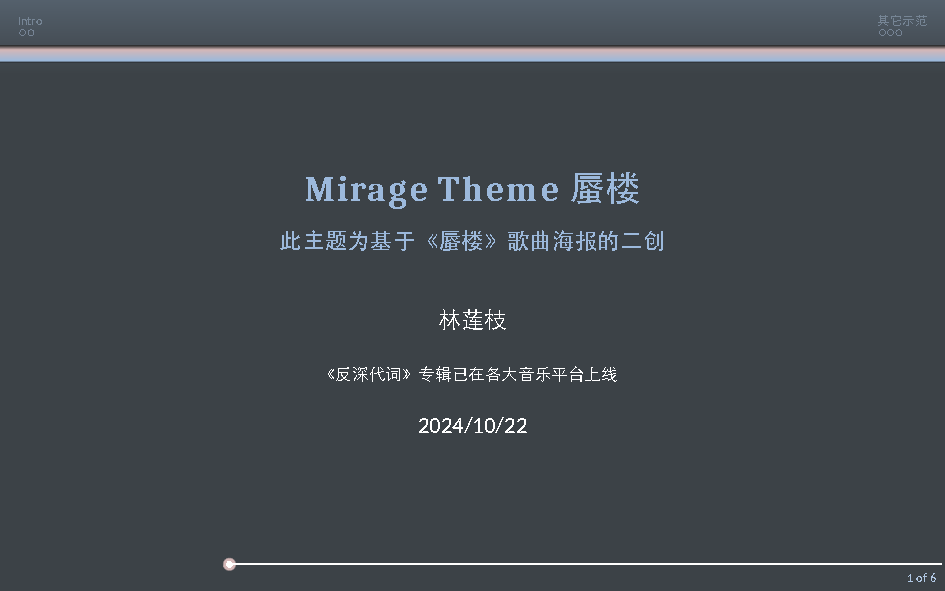
\includegraphics[page=1,width=.495\hsize]{mirage-beamer-zh.pdf}
\includegraphics[page=5,width=.495\hsize]{mirage-beamer-zh.pdf}
\end{center}
    
\begin{paracol}{2}
\section{Basic Usage}

Two modes are available: the default has a dark look, while the
\texttt{light} mode may be more suitable for printouts.

\switchcolumn

\section{基本用法}

两种模式可选:默认模式颜色深沉,\texttt{light}模式颜色较浅,较适合列印。详细使用方法可参考示范 .tex 文档。

\end{paracol}

\begin{center}
\begin{BVerbatim}
\usetheme{Mirage}  OR  \usetheme[light]{Mirage}
\end{BVerbatim}
\end{center}


\begin{paracol}{2}
The English sample files \texttt{*-en.tex} can be compiled with \hologo{pdfLaTeX}, \hologo{XeLaTeX} or \hologo{LuaLaTeX}; but compile the Chinese sample files \texttt{*-zh.tex} with \hologo{XeLaTeX}. Compile twice to get the correct total number of frames in the footer.

\switchcolumn

英文示范文档 \texttt{*-en.tex} 可用 \hologo{pdfLaTeX}, \hologo{XeLaTeX} 或 \hologo{LuaLaTeX}
编译。中文示范文档 \texttt{*-zh.tex} 请用中文编译。页脚里的幻灯片帧数需多次编译才能正确显示。

\switchcolumn*
\setlength{\fboxsep}{0pt}

\begin{center}
\foreach \n in {1,...,6} {\fbox{\includegraphics[page=\n,width=.49\hsize]{mirage-beamer-zh.pdf}} }
\end{center}

\switchcolumn

\begin{center}
\foreach \n in {1,...,6} {\fbox{\includegraphics[page=\n,width=.49\hsize]{mirage-beamer-en.pdf}} }
\end{center}

\switchcolumn*


\section{Posters}

With some modificatons, the Mirage theme can be used for creating posters  the \texttt{beamerposter} package. See sample files \texttt{mirage-poster-en.tex} and \texttt{mirage-poster-zh.tex} for examples.

\switchcolumn

\section{海报}

“蜃楼”主题也可以和\texttt{beamerposter}搭配使用制作海报(一些设置需些许修改),请参照\texttt{mirage-poster-zh.tex}及\texttt{mirage-poster-en.tex}.

\switchcolumn*

\begin{center}
\fbox{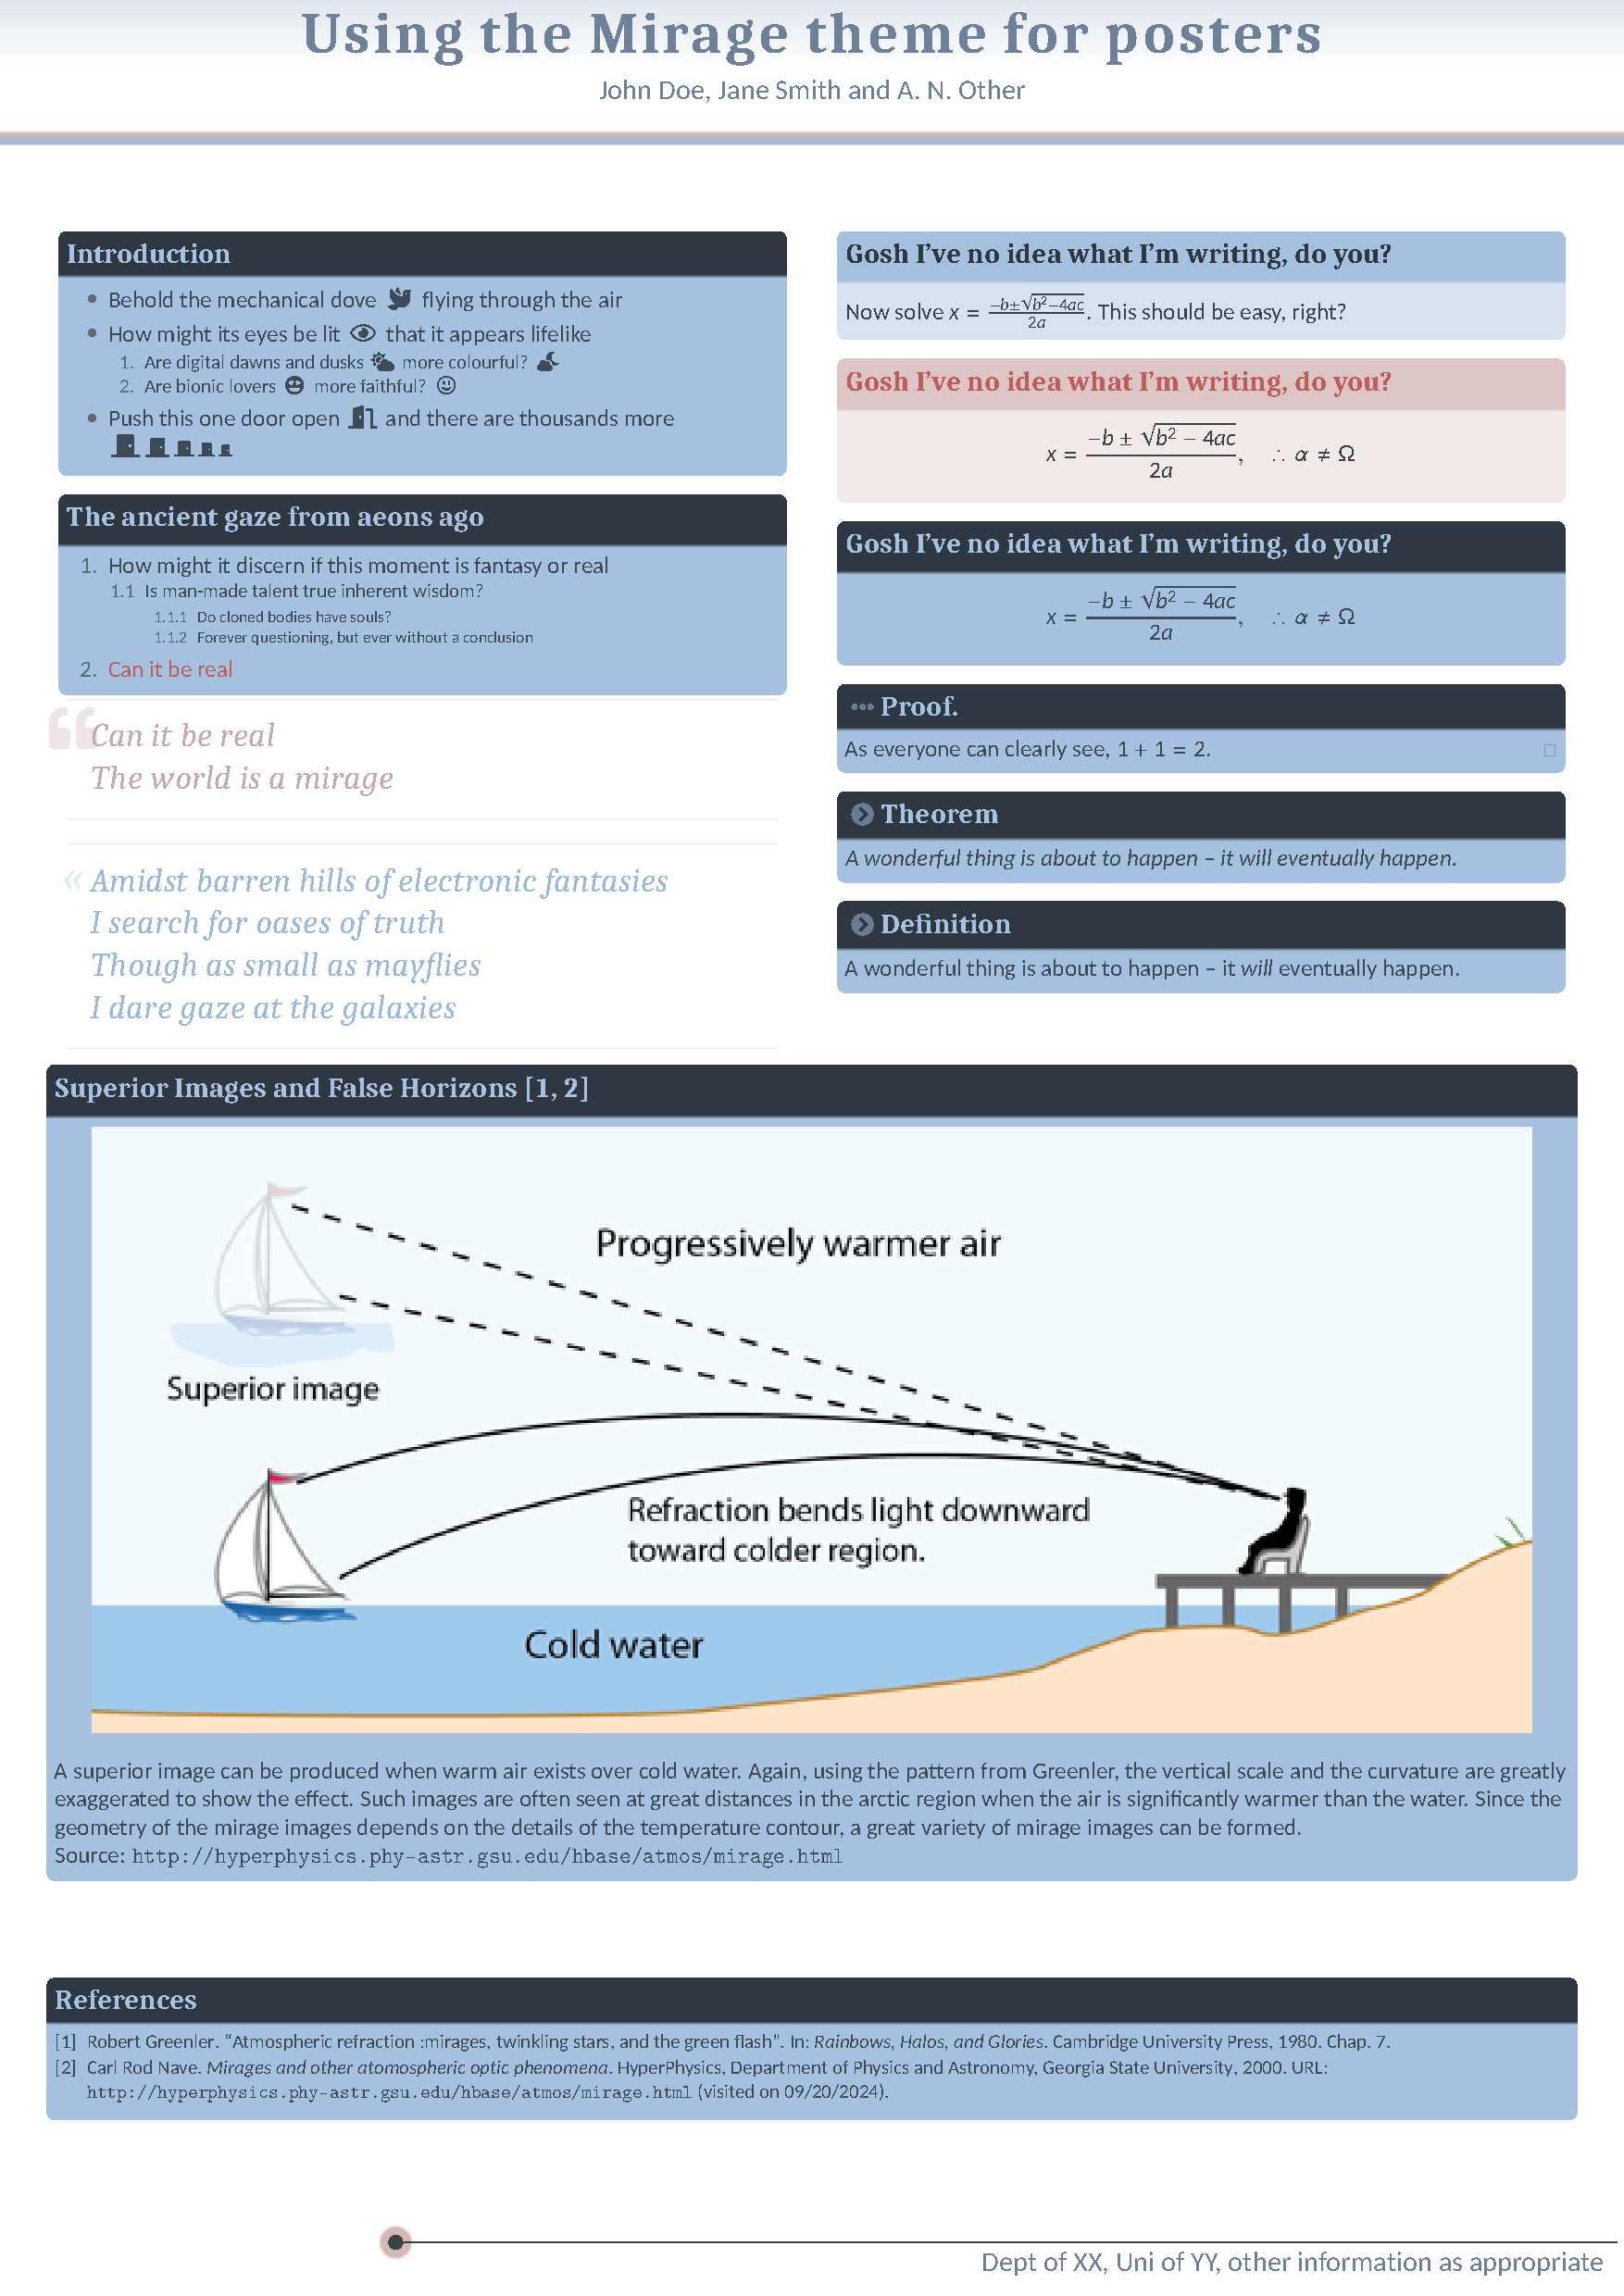
\includegraphics[width=.8\hsize]{mirage-poster-en.pdf}}
\end{center}

\switchcolumn

\begin{center}
\fbox{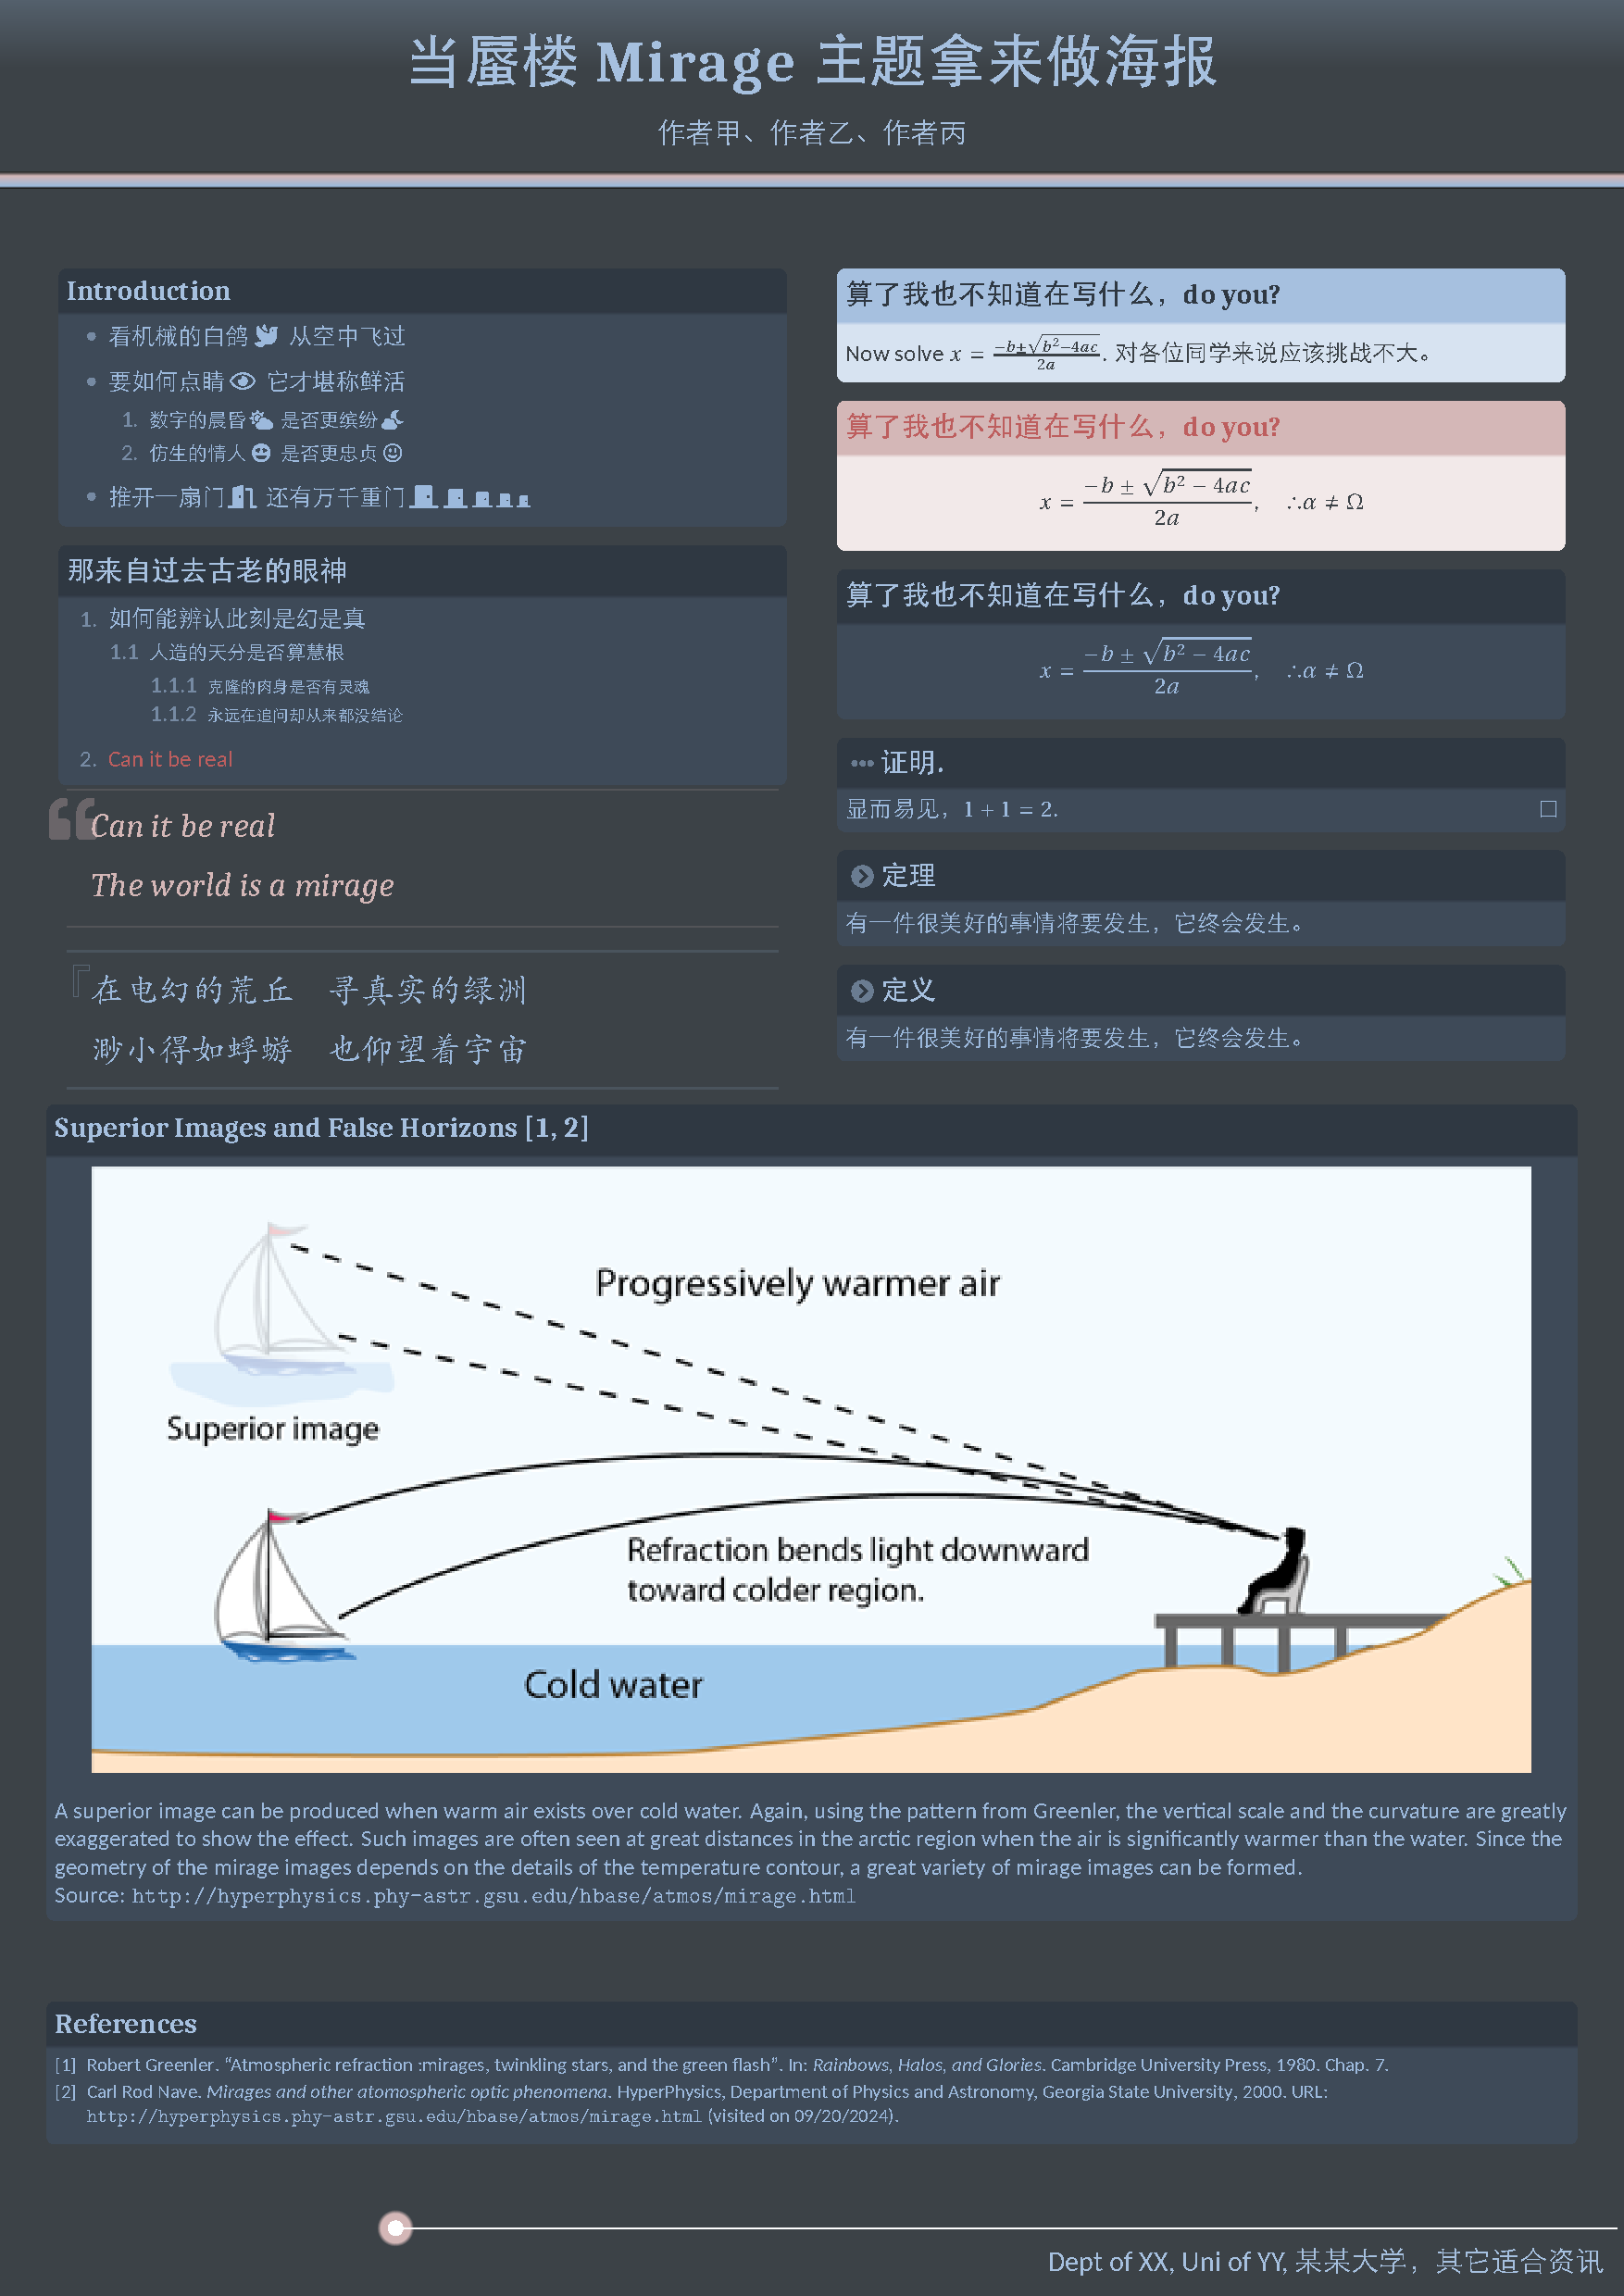
\includegraphics[width=.8\hsize]{mirage-poster-zh.pdf}}
\end{center}

\switchcolumn*

\section{Some simple customisationoptions}

\begin{itemize}
\item The Mirage theme itself doesn't set any body fonts, so you can load your own preferred fonts in your \texttt{.tex} files.

\item  The sample \texttt{.tex} files load the font packages \texttt{caladea}, \texttt{carlito}, \texttt{newtxsf} for the English (\hologo{pdfLaTeX}) samples, and \texttt{Fira Math} for the Chinese (\hologo{XeLaTeX}) samples. You can change these as you like.

\item \texttt{pullquote} used in frame 4 is a custom environment. You can change its beamer font and color, or re-define the \verb|\MiragePullquoteOpen| marker (see frame 4).

\item  Other markers that can be \verb|\renewcommand|:
\begin{itemize}[nosep]
  \item \verb|\MirageFrametitlePrefix|
  \item \verb|\MirageProofPrefix| 
  \item \verb|\MirageTheoremPrefix|
\end{itemize} 
for prefix icons of the frame title, \texttt{proof} block title and \texttt{theorem}-like block titles. (See commented code before frame 5.)

\item The Mirage theme loads \texttt{fontawesome5}, so you can use
icons provided by this package.

\item \verb|\MirageGlowRadius| is a length controlling the size of the glowy circle in the footline; especially useful when creating posters with \texttt{beamerposter}.
\end{itemize}

\switchcolumn

\section{一些可调整的元素}
\begin{itemize}
\item “蜃楼”本身并没有设置任何字体,用户可以自行在\texttt{.tex}导言曲加载自己喜欢的宏包或设置字体。

\item  示范的 \texttt{.tex} 档案导言区加载了\texttt{caladea}、\texttt{carlito}、 \texttt{newtxsf} (仅限英文\hologo{pdfLaTeX}示范文档) 、\texttt{Fira Math} (仅限中文\hologo{XeLaTeX}示范文档)。这些都是可以自行更换的!

\item 第4帧幻灯片里用的\texttt{pullquote}环境是“蜃楼”主题自定义的。它的beamer font、color都是可以更换的, 也可重新定义前缀装饰 \verb|\MiragePullquoteOpen| marker(详见第4帧幻灯片示范代码)。

\item  其它可以 \verb|\renewcommand|的装饰:
\begin{itemize}[nosep]
    \item \verb|\MirageFrametitlePrefix|
    \item \verb|\MirageProofPrefix|
    \item \verb|\MirageTheoremPrefix| 
\end{itemize} 
这些是frame title、\texttt{proof} block title 以及\texttt{theorem}之类block titles的前缀装饰。(详见第5帧幻灯片之前的注释)

\item “蜃楼”主题已加载\texttt{fontawesome5}宏包,可以尽情使用此宏包提供的符号。

\item \verb|\MirageGlowRadius| 是用来控制页脚的小光球半径的length;制作海报时可以酌量加大。
\end{itemize}

\end{paracol}

\section{Revision History}
\begin{description}
\item[v1.0 (2024/04/14)] Initial commit.
\item[v1.01 (2024/09/18)] Adds beamerposter example and some updates for some easier customisations.
\item[v1.1 (2024/10/24)] Reorganises sample .tex files and documentations; submitted to CTAN.
\item[v1.1.1 (2025/01/19)] Bug fix: added missing second argument to \verb|\addtobeamertemplate{frametitle}|.
\end{description}
\end{document}